\documentclass{article}
\usepackage{graphicx} % Required for inserting images
\graphicspath{{Images/}}
\usepackage[utf8]{inputenc}
\usepackage{multicol}
\usepackage{amsthm}
\usepackage{amsmath}
\usepackage{xcolor}
\usepackage{subfigure}


\newtheorem{definition}{Definition}[section]
\newtheorem{remark}{Remarque}[section]
\newtheorem{theorem}{Théorème}[section]
\newtheorem{strat}{Stratégie de résolution}[section]

\title{Algèbre Linéaire}
\author{Laura Paraboschi / Simon Lefort }
\date{BA1 - IN}

\begin{document}

\maketitle

\section{Equations linéaires}
\begin{definition}
    Une équation linéaire est de la forme :
    \[ a_1x_1 + a_2x_2 + ... + a_nx_n = b \]
    Pour des nombres \( a_1, \ a_2, \ ..., \ a_n \ \)et b indépendants des variables
\end{definition}
\begin{figure}[h]
    \centering
    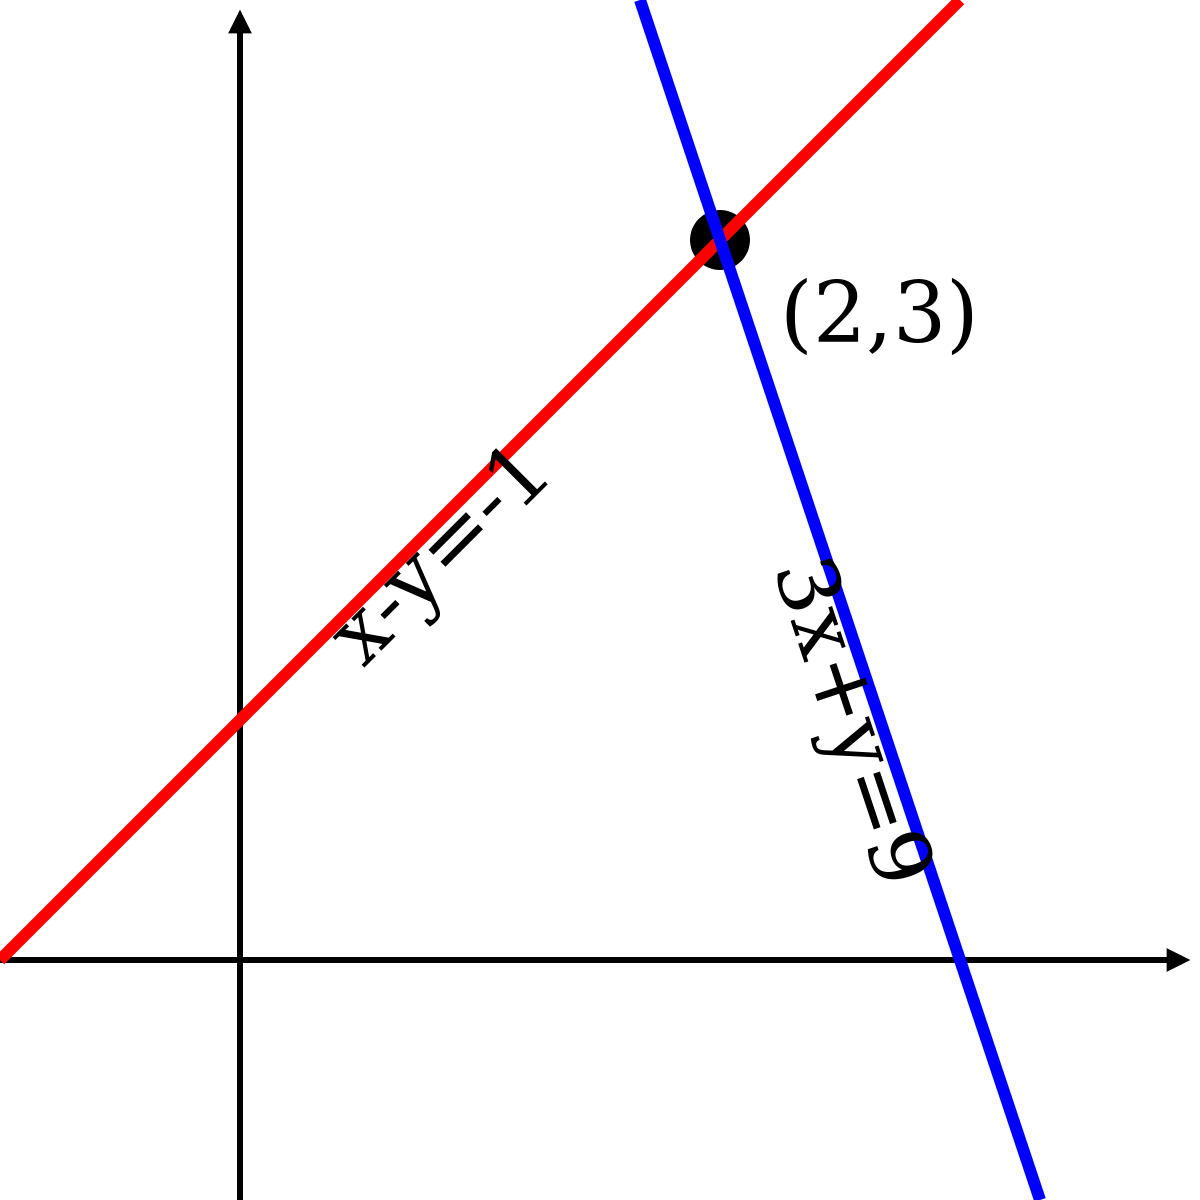
\includegraphics[width=4cm]{Images/1200px-Intersecting_Lines.svg.png}
    \caption{à 2 inconnues}
    \label{fig:Graphe 2 inconnues}
\end{figure}
\begin{definition}
    Un système linéaire est une collection de une ou plusieurs équations linéaires
    \begin{equation}
        \begin{cases}
            a_{1,1}x_1 + ... + a_{1,n}x_n = b_1\\
            a_{m,1}x_1 + ... + a_{m,n}x_n = b_m
        \end{cases}
    \end{equation}
\end{definition}
\begin{theorem}
    Un système linéaire a zéro, une ou une infinité de solutions
\end{theorem}
\begin{theorem}[Opérations élémentaires]
    Ces opérations ne changent pas les solutions du système :
    \begin{itemize}
        \item Permuter 2 équations
        \item Multiplier une équation par un nombre non nul
        \item Soustraire un multiple d'une équation à une autre
    \end{itemize}
\end{theorem}
\begin{definition}
    Pour une matrice de taille m \(\times\) n, on appelle \textcolor{red}{coefficient principal} d'une ligne non-nulle le coefficient non-nul le plus à gauche dans la ligne
\end{definition}
Une matrice est sous forme \underline{échelonnée} si
\begin{enumerate}
    \item Toutes les lignes non-nulles (s'il y en a) sont en bas
    \item Le coefficient principal de toute ligne se trouve à droite du coefficient principal de la ligne au dessus, \underline{et}
    \item Tous les coefficients d'une colonne sous un coefficient principal sont nuls
    \[ \begin{pmatrix}
            \textcolor{red}{a_{1,1}} & a_{1,2} & a_{1,3} & b_1 \\ 
            0 & \textcolor{red}{a_{2,2}} & a_{2,3} & b_2\\
            0 & 0 & 0 & 0
        \end{pmatrix} \]
\end{enumerate}
Une matrice qui satisfait \underline{en plus} les deux conditions ci-dessous est sous forme \underline{échelonnée réduite} :
\begin{enumerate}
    \item Le coefficient principal de chaque ligne vaut 1 \underline{et}
    \item Les coefficients principaux sont les seuls éléments non-nuls de leur colonne
    \[ \begin{pmatrix}
            \textcolor{red}{1} & 0 & a_{1,3} & b_1 \\ 
            0 & \textcolor{red}{1} & a_{2,3} & b_2\\
            0 & 0 & 0 & 0
        \end{pmatrix} \]
\end{enumerate}
\begin{definition}
    Deux matrices sont \underline{équivalentes par les lignes} si on peut obtenir l'une à partir de l'autre via une séquence d'opérations élémentaires sur les lignes
\end{definition}
\begin{remark}
    Toute matrice non-nulle est équivalente par les lignes avec plusieurs  matrices échelonnées
\end{remark}
\begin{theorem}
    Toute matrice échelonnée est équivalente par les lignes à \underline{exactement une} matrice échelonnée réduite
\end{theorem}
\begin{strat}
    Résoudre un système d'équations
    \begin{enumerate}
        \item Ecrire la matrice augmentée du système
        \[ \begin{pmatrix}
            a_{1,1} & a_{1,2} & a_{1,3} & b_1 \\ 
            a_{2,1} & a_{2,2} & a_{2,3} & b_2\\
            a_{3,1} & a_{3,2} & a_{3,3} & b_3
        \end{pmatrix} \]
        \item Mettre la matrice sous forme échelonnée à l'aide des opérations élémentaires
        \[ \begin{pmatrix}
            a_{1,1} & a_{1,2} & a_{1,3} & b_1 \\ 
            0 & a_{2,2} & a_{2,3} & b_2\\
            0 & 0 & a_{3,3} & b_3
        \end{pmatrix} \]
        \begin{itemize}
            \item Si \( a_{3,3} = 0\) et \(b_3 = 0 \), alors le système aura une infinité de solution avec une variable libre
            \item Si \( a_{3,3} = 0\) et \(b_3 \neq 0 \), alors le système n'aura aucune solution
        \end{itemize}
        \item Continuer de façon à obtenir une matrice échelonnée réduite
        \[ \begin{pmatrix}
            1 & 0 & 0 & b_1 \\ 
            0 & 1 & 0 & b_2\\
            0 & 0 & 1 & b_3
        \end{pmatrix} \]
        \item Réécrire le système d'équation
        \item Exprimer chaque variable liée en fonction des variables libres
    \end{enumerate}
\end{strat}
\section{Equations vectorielles}
\subsection{Propriétés algébriques de \( \mathbf{R}^n \) }
\begin{multicols}{2}
    \begin{itemize}
        \item \( \overrightarrow{u} + \overrightarrow{v} =  \overrightarrow{v} + \overrightarrow{u} \)
        \item \( \overrightarrow{u} + \overrightarrow{0} = \overrightarrow{u}\)
        \item \(\overrightarrow{u} + \overrightarrow{-u} = \overrightarrow{0}\)
    \end{itemize}
\columnbreak
\begin{itemize}
    \item \( a(\overrightarrow{u} + \overrightarrow{v}) = a\overrightarrow{u}  + a\overrightarrow{v} \)
    \item \( (a + b)\overrightarrow{u} = a\overrightarrow{u} + b\overrightarrow{u} \)
    \item \(a(b\overrightarrow{u}) = (ab)\overrightarrow{u}\)
\end{itemize}
\end{multicols}
\subsection{Combinaison linéaire}
\( \overrightarrow{y} = c_1\overrightarrow{v}_1 + c_2\overrightarrow{v}_2 ... + c_p\overrightarrow{v}_p \) 
\begin{definition}
    \(Vect(\overrightarrow{v}_1, ..., \overrightarrow{v}_p)\) est le sous ensemble de \(R^n\) engendré par les vecteurs
\end{definition}
\begin{figure}[htp]
    \centering
    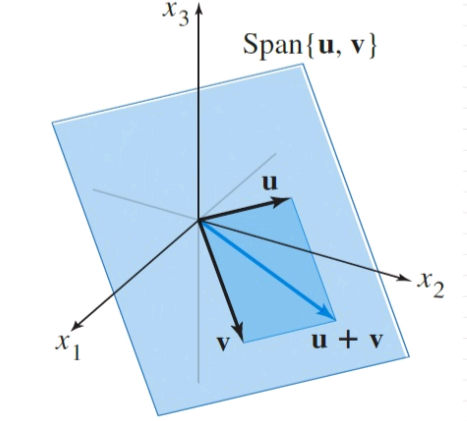
\includegraphics[width=4cm]{Images/Span.png}
    \caption{Vect()}
    \label{fig:span}
\end{figure}
On peut résoudre : \( A\overrightarrow{x} = \overrightarrow{b}\) pour trouver les composantes \(C_x\) (solution particulière) ou \( A\overrightarrow{x} = \overrightarrow{b}\) pour trouver la solution homogène \newpage
Cela donnera une solution de la forme : \(\begin{pmatrix}
    x \\
    y \\
    0
\end{pmatrix} + t\begin{pmatrix}
    a \\
    b \\
    1
\end{pmatrix} \)  pour \(x_3\) libre \\
\begin{figure}[htp]
    \centering
    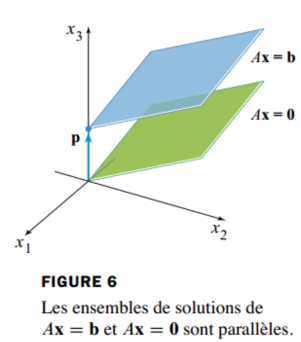
\includegraphics[width=5cm]{Images/Paralleles.png}
    \label{fig:parallele}
\end{figure}
\subsection{Indépendance linéaire}
On dit qu'une famille de vecteurs est linéairement indépendante si :
\[ x_1v_1 + x_2v_2 + ... + x_nv_n = 0\]
admet la solution triviale comme unique solution (ou liés si les \(x_n\) ne sont pas tous nuls en même temps)\\
On peut résoudre le système homogène \( A\overrightarrow{x} = \overrightarrow{0}\) pour savoir si nos vecteurs sont linérairement dépendants : \\
Si la seule solution possible est la solution triviale (0) alors les vecteurs engendrent \(R^x\) (si nous avons suffisament de vecteurs) et on peut créer n'importe quel vecteur dans la dimension x
\begin{figure}[htp]
    \centering
    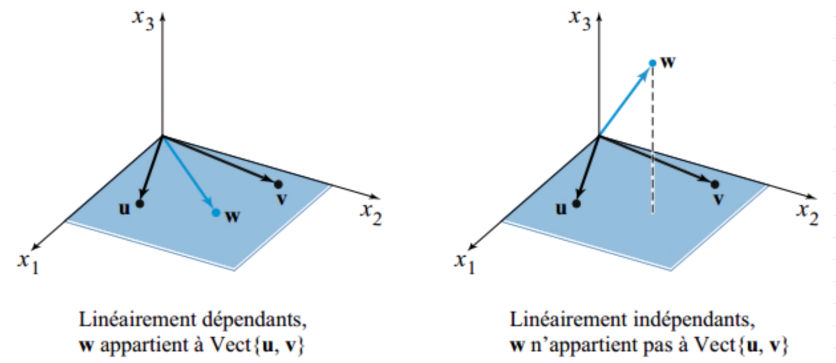
\includegraphics[width=12cm]{Images/linéarité.png}
    \label{fig:linearite}
\end{figure}
\begin{remark}
    Si on a p vecteurs dans une dimension \(R^n\) avec n \(>\) p, alors la famille de vecteurs est forcément linéairement dépendante 
\end{remark}
\end{document}
